\chapter{Non-relational DBMS inside VO}

Typically, modern relational databases have shown little efficiency in certain applications using intensive data, like indexing of a large number of documents, sites rendering with high traffic, and streaming sites. Typical RDBMS implementations are tuned either for small but frequent reads and writes or a large set of transactions that have few write accesses. On the other hand NoSQL can serve load lots of reads and writes. A non-relational database just stores data without explicit and structured mechanisms to link data from different buckets to one another. \newline

IVOA has a standard called Astronomical Data Query Language (ADQL) that users do not necessarily need to know, because he can pose a query with a GUI, as long as the query is translated into standard ADQL. The receiving service likewise converts the standard ADQL into whatever its own database servers need, but always inside relational model. For the reasons stated in chapter \ref{theproblem}, we propose the use of a different approach, the NoSQL technology.


\section{NoSQL}

A non-relational database just stores data without explicit and structured mechanisms to link data from different buckets to one another. \newline

NoSQL implementations used in the real world include 3TB Digg green markers (indicated to highlight the stories voted by others in the social network), the 6 TB of "ENSEMBLE" European Commission database used in comparing models and air quality, and the 50 TB of Facebook inbox search. \newline

NoSQL architectures often provide limited consistency, such as events or transactional consistency restricted to only data items. Some systems, however, provide all guarantees offered by ACID systems by adding an intermediate layer. There are two systems that have been deployed and provide for storage of snapshot isolation column: Google Percolator (based on BigTable system) and Hbase transactional system developed by the University of Waterloo. These systems use similar concepts in order to achieve distributed multiple rows ACID transactions with snapshot isolation guarantees for the underlying storage system in that column, wit no extra overhead in data management, no system deployment middleware or any maintenance introduced by middleware layer. \newline

Quite NoSQL systems employ a distributed architecture, maintaining data redundantly on multiple servers, often using distributed hash table. Thus, the system may actually escale adding more servers, and thus a server failure may be tolerated. \newline

There are different NoSQL DBs for different projects:

\begin{itemize}

\item Document oriented

  \begin{itemize}
    \item CouchDB
    \item MongoDB
    \item RavenDB
    \item IBM Lotus Domino
  \end{itemize}

\item Graph oriented

  \begin{itemize}
    \item Neo4j
    \item AllegroGraph
    \item InfiniteGraph
    \item Sones GraphDB
    \item HyperGraphDB
  \end{itemize}

\item Key-value oriented

  \begin{itemize}
    \item Cassandra
    \item BigTable
    \item Dynamo (Amazon)
    \item MongoDB
    \item Project Voldemort (LinkedIn)
  \end{itemize}

\item Multivalue

  \begin{itemize}
    \item OpenQM
  \end{itemize}  

\item Object Oriented
  
  \begin{itemize}
    \item Zope Object Database
    \item db4o
    \item GemStone S
    \item Objectivity/DB
  \end{itemize}

\item Tabular

  \begin{itemize}
    \item HBase
    \item BigTable
    \item LevelDB (BigTable open version)
    \item Hypertable
  \end{itemize}
  

\end{itemize}

They run on clusters of inexpensive machines.



\section{MongoDB: a document oriented database}

MongoDB (from "humongous") is an open source document-oriented database system developed and supported by 10gen. It is part of the NoSQL family of database systems. Instead of storing data in tables as is done in a "classical" relational database, MongoDB stores structured data as JSON-like documents with dynamic schemas (MongoDB calls the format BSON), making the integration of data in certain types of applications easier and faster. \newline

As an example, we show some JSON code inserting a document in a Mongo DB:
\begin{lstlisting}
db.columns.insert( {
		table_name: "TAP_SCHEMA.schemas",
		column_name: "schema_name",
		utype: null,
		ucd: null,
		unit: null,
		description: "schema name for reference to TAP_SCHEMA.schemas",
		datatype: "VARCHAR",
		size: 64,
		principal: 1,
		indexed: 0,
		std: 0
	}
);
\end{lstlisting} 


10gen began Development of MongoDB in October 2007 and was not created to be just another database that tries to do everything for everyone. Instead, MongoDB was created to work with documents rather than rows, was extremely fast, massively scalable, and easy to use. In order to accomplish this, some features were excluded, namely support for transactions. \newline

%\begin{shaded}
A document database is more like a collection of documents. Each entry is a document, and each one can have its own structure. If you want to add a field to an entry, you can do so without affecting any other entry.
%\end{shaded} 

\begin{table}
\begin{center}
\begin{tabular}{|l|l|}
\hline
\textbf{Relational} & \textbf{Document oriented} \\ 
\hline
Table & Collection\\
\hline
Row & Document\\
\hline
Column & Field \\
\hline
\end{tabular}
\end{center}
\caption{Differences between relational and NoSQL terms}
\end{table}




\subsection{Main features}

\begin{itemize}

\item \textbf{Ad hoc queries} 
MongoDB supports search by field, range queries, regular expression searches. Queries can return specific fields of documents and also include user-defined JavaScript functions.

\item \textbf{Indexing} 
Any field in a MongoDB document can be indexed (indices in MongoDB are conceptually similar to those in RDBMSes). Secondary indices are also available.

\item \textbf{Replication} 
MongoDB supports master-slave replication. A master can perform reads and writes. A slave copies data from the master and can only be used for reads or backup (not writes). The slaves have the ability to select a new master if the current one goes down.

\item \textbf{Load balancing} 
MongoDB scales horizontally using sharding.[9] The developer chooses a shard key, which determines how the data in a collection will be distributed. The data is split into ranges (based on the shard key) and distributed across multiple shards. (A shard is a master with one or more slaves.)
MongoDB can run over multiple servers, balancing the load and/or duplicating data to keep the system up and running in case of hardware failure. Automatic configuration is easy to deploy and new machines can be added to a running database.

\item \textbf{File storage} 
MongoDB could be used as a file system, taking advantage of load balancing and data replication features over multiple machines for storing files.
This function, called GridFS,[10] is included with MongoDB drivers and available with no difficulty for development languages (see "Language Support" for a list of supported languages). MongoDB exposes functions for file manipulation and content to developers. GridFS is used, for example, in plugins for NGINX and lighttpd. In a multi-machine MongoDB system, files can be distributed and copied multiple times between machines transparently, thus effectively creating a load balanced and fault tolerant system.

\item \textbf{Aggregation} 
MapReduce can be used for batch processing of data and aggregation operations. The aggregation framework enables users to obtain the kind of results for which the SQL GROUP BY clause is used.

\item \textbf{Server-side JavaScript execution} 
JavaScript can be used in queries, aggregation functions (such as MapReduce), are sent directly to the database to be executed.

\item \textbf{Capped collections} 
MongoDB supports fixed-size collections called capped collections. This type of collection maintains insertion order and, once the specified size has been reached, behaves like a circular queue.

Once we have seen the main features of MongoDB, we can move on to the language itself.
\end{itemize}


\subsection{The basics}

We must know four concepts to dig into MongoDB's world:

\begin{itemize}
\item Database: this concept is much like the RDBM counterpart.
\item Collection: we can see a collection and a table as the same thing.
\item Document: its equivalent in RDBM is the row, and a document is made up of fields.
\item Field: is a lot like a column.
\end{itemize}


\begin{figure}[H]
\centering
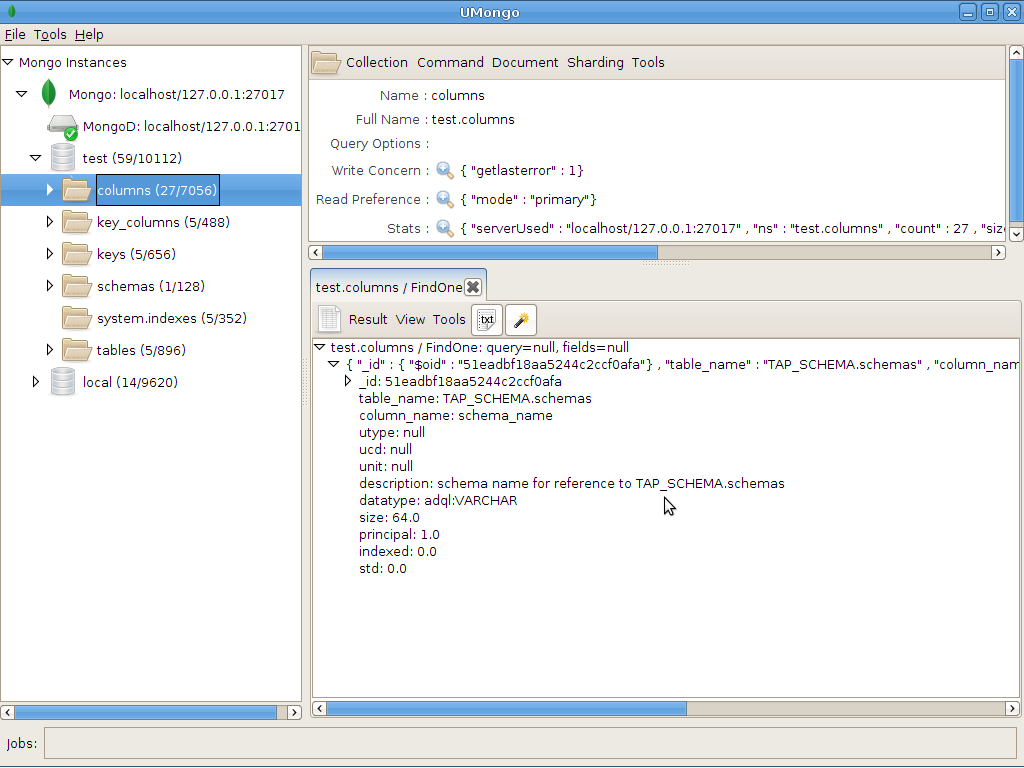
\includegraphics[width=11cm,height=8cm]{images/mongo_dia.png}
\caption{Tree View for Tap Schema in MongoVue}
\end{figure}


\section{Advantages and uncertainties of NoSQL}

\begin{itemize}

\item \textbf{Elastic scaling}

For years, database administrators have relied on scale up — buying bigger servers as database load increases — rather than scale out — distributing the database across multiple hosts as load increases. However, as transaction rates and availability requirements increase, and as databases move into the cloud or onto virtualized environments, the economic advantages of scaling out on commodity hardware become irresistible.

RDBMS might not scale out easily on commodity clusters, but the new breed of NoSQL databases are designed to expand transparently to take advantage of new nodes, and they’re usually designed with low-cost commodity hardware in mind.


\item \textbf{Big data}

Just as transaction rates have grown out of recognition over the last decade, the volumes of data that are being stored also have increased massively. O’Reilly has cleverly called this the “industrial revolution of data.” RDBMS capacity has been growing to match these increases, but as with transaction rates, the constraints of data volumes that can be practically managed by a single RDBMS are becoming intolerable for some enterprises. Today, the volumes of “big data” that can be handled by NoSQL systems, such as Hadoop, outstrip what can be handled by the biggest RDBMS.


\item \textbf{No need for DBAs}

Despite the many manageability improvements claimed by RDBMS vendors over the years, high-end RDBMS systems can be maintained only with the assistance of expensive, highly trained DBAs. DBAs are intimately involved in the design, installation, and ongoing tuning of high-end RDBMS systems.

NoSQL databases are generally designed from the ground up to require less management:  automatic repair, data distribution, and simpler data models lead to lower administration and tuning requirements — in theory. In practice, it’s likely that rumors of the DBA’s death have been slightly exaggerated. Someone will always be accountable for the performance and availability of any mission-critical data store.


\item \textbf{Economics}

NoSQL databases typically use clusters of cheap commodity servers to manage the exploding data, while RDBMS tends to rely on expensive proprietary servers and storage systems. The result is that the cost per gigabyte or transaction/second for NoSQL can be many times less than the cost for RDBMS, allowing you to store and process more data at a much lower price point.


\item \textbf{Flexible data models}

Change management is a big headache for large production RDBMS. Even minor changes to the data model of an RDBMS have to be carefully managed and may necessitate downtime or reduced service levels.

NoSQL databases have far more relaxed — or even nonexistent — data model restrictions. NoSQL Key Value stores and document databases allow the application to store virtually any structure it wants in a data element. Even the more rigidly defined BigTable-based NoSQL databases (Cassandra, HBase) typically allow new columns to be created without too much fuss.

The result is that application changes and database schema changes do not have to be managed as one complicated change unit. In theory, this will allow applications to iterate faster, though,clearly, there can be undesirable side effects if the application fails to manage data integrity.

\end{itemize}


NoSQL systems have generated a lot of enthusiasm but there are still a lot of questions about its future:

\begin{itemize}

\item \textbf{Maturity}

RDBMS systems have been around for a long time. NoSQL advocates will argue that their advancing age is a sign of their obsolescence, but for most CIOs, the maturity of the RDBMS is reassuring. For the most part, RDBMS systems are stable and richly functional. In comparison, most NoSQL alternatives are in pre-production versions with many key features yet to be implemented. Living on the technological leading edge is an exciting prospect for many developers, but enterprises should approach it with extreme caution.

\item \textbf{Support}

Enterprises want the reassurance that if a key system fails, they will be able to get timely and competent support. All RDBMS vendors go to great lengths to provide a high level of enterprise support.

In contrast, most NoSQL systems are open source projects, and although there are usually one or more firms offering support for each NoSQL database, these companies often are small start-ups without the global reach, support resources, or credibility of an Oracle, Microsoft, or IBM.
 
\item \textbf{Analytics and business intelligence}

NoSQL databases have evolved to meet the scaling demands of modern Web 2.0 applications. Consequently, most of their feature set is oriented toward the demands of these applications. However, data in an application has value to the business that goes beyond the insert-read-update-delete cycle of a typical Web application. Businesses mine information in corporate databases to improve their efficiency and competitiveness, and business intelligence (BI) is a key IT issue for all medium to large companies.

NoSQL databases offer few facilities for ad-hoc query and analysis. Even a simple query requires significant programming expertise, and commonly used BI tools do not provide connectivity to NoSQL.

Some relief is provided by the emergence of solutions such as HIVE or PIG, which can provide easier access to data held in Hadoop clusters and perhaps eventually, other NoSQL databases. Quest Software has developed a product — Toad for Cloud Databases — that can provide ad-hoc query capabilities to a variety of NoSQL databases.

\item \textbf{Administration}

The design goals for NoSQL may be to provide a zero-admin solution, but the current reality falls well short of that goal. NoSQL today requires a lot of skill to install and a lot of effort to maintain.

\item \textbf{Expertise}

There are literally millions of developers throughout the world, and in every business segment, who are familiar with RDBMS concepts and programming. In contrast, almost every NoSQL developer is in a learning mode. This situation will address naturally over time, but for now, it is by far easier to find experienced RDBMS programmers or administrators than NoSQL experts.

\end{itemize}


\section{A FITS alternative with MongoDB}

A very important issue when working with FITS format is the great amount of possible key-value pairs in FITS headers. A possible solution for this problem could be use the features of MongoDB to translate FITS keywords into collections. So, we could create as much documents as needed, and storing them into MongoDB. Should we need to create supertypes of FITS headers, relations are also available in MongoDB through document linking (with no physical restriction in the sense of relational constraint).

%TODO: ejemplo de conversión de fits a documentos de Mongo